\section{Dataflow Engine for Filtering and Dropping}
\label{sec:arch}

% % Overview of inserting dataflow engine between main and monitoring core
% \begin{figure}
%   \begin{center}
%     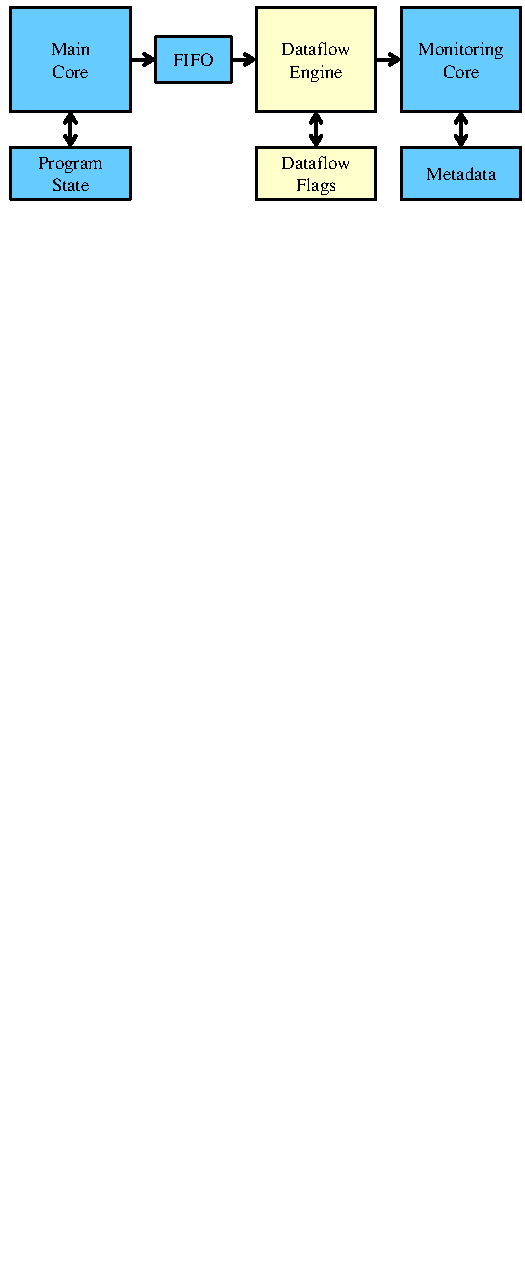
\includegraphics[width=\linewidth]{figs/dataflow_overview.pdf}
%     \vspace{-0.2in}
%     \caption{Overview of architecture for reduced and adjustable monitoring
%     overheads.}
%     \label{fig:arch.overview} 
%     \vspace{-0.1in}
%   \end{center}
% \end{figure}

% Overview of full architecture
\begin{figure}
  \begin{center}
    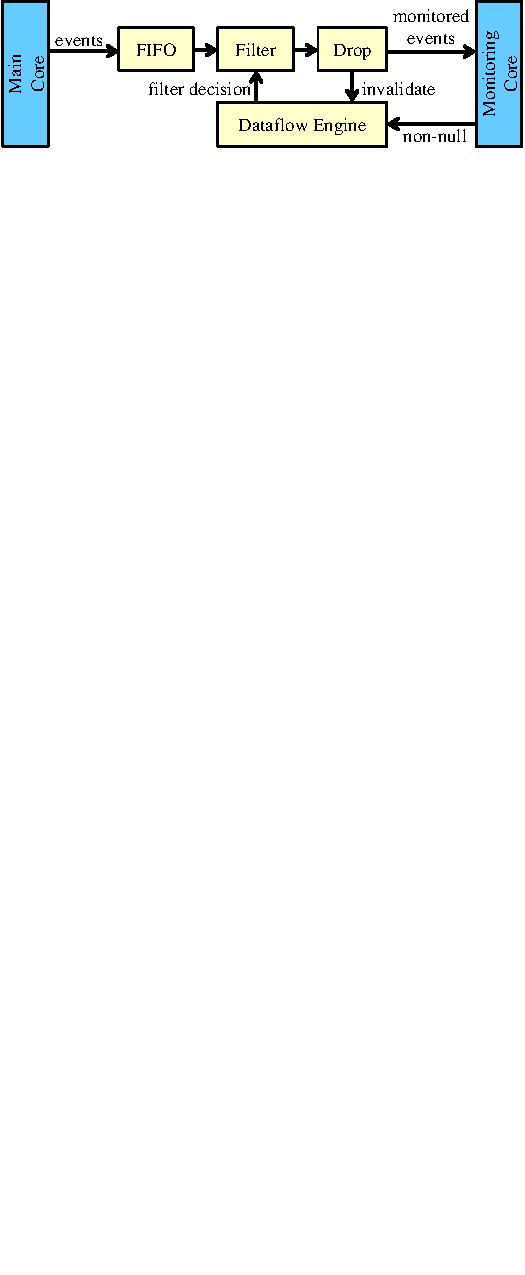
\includegraphics[width=\columnwidth]{figs/architecture_overview.pdf}
    \vspace{-0.2in}
    \caption{Block diagram of architecture for monitoring with reduced and adjustable overheads.}
    \label{fig:arch.overview}
    \vspace{-0.1in}
  \end{center}
\end{figure}

For both filtering and partial monitoring, we need to be able to track
dataflows. For filtering, we need to track the dataflow of null metadata and
for partial monitoring, we need to track the dataflow of invalid metadata.
In this section, we will describe our dataflow-guided hardware architecture for
enabling both filtering and partial monitoring.
Figure~\ref{fig:arch.overview} shows a high-level block diagram of the
architecture. The basic idea is to insert this dataflow-guided hardware between the main core and
the monitoring core. This hardware reduces the number of monitoring events that reach
the monitoring core in order to reduce monitoring overheads.

As in the baseline architecture from Section~\ref{sec:monitoring}, events from
the main core are first buffered in a FIFO. 
Events are first filtered out based on whether they correspond to null or
invalid metadata. A hardware dataflow engine is used to track the flow of null
and invalid metadata and decide whether
specific events can be filtered out.
Next, if the event is not filtered out, then we
check whether the event should be dropped in order to stay within the specified
overhead budget. Whenever an event is dropped, its corresponding metadata is
marked and tracked as invalid by the dataflow engine. The
dropping decision hardware is described in detail in Section~\ref{sec:policies}.
Finally, if the event is not filtered or dropped, then it is forwarded to the
monitoring core to be processed.

\subsection{Filtering Using the Dataflow Engine}
\label{sec:arch.dataflow}

% Detailed architecture of dataflow engine
\begin{figure*}
  \begin{center}
    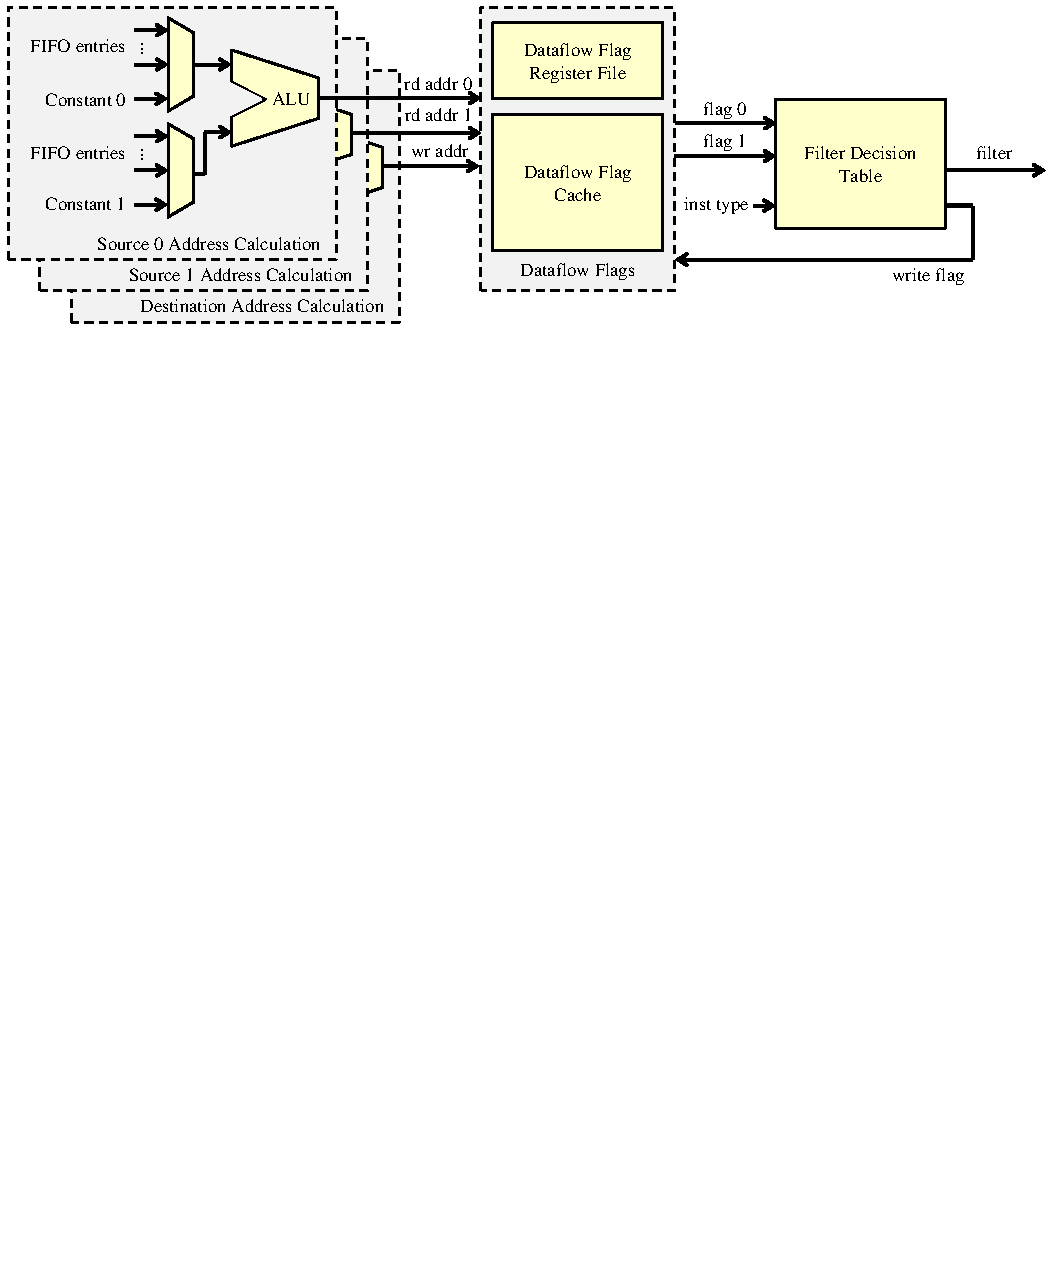
\includegraphics[width=\linewidth]{figs/dataflow_architecture.pdf}
    \vspace{-0.2in}
    \caption{Hardware architecture of the dataflow engine.}
    \label{fig:arch.dataflow} 
    \vspace{-0.1in}
  \end{center}
\end{figure*}

% Overview
In order to perform filtering, we need to be able to identify and track flows
of null metadata. Similarly, for partial monitoring,
 we need to be able to track the flow of invalid metadata. In
order to efficiently track these flows, we use a dedicated hardware
dataflow engine. A block diagram of the dataflow engine is shown in
Figure~\ref{fig:arch.dataflow}.

% Flags and flag storage
In order to track both null metadata flows and invalid metadata flows, the
dataflow engine tracks the flow of 2-bit flags. One bit is used to
mark metadata as null while the other bit is used to mark metadata as invalid.
Monitoring schemes typically keep metadata corresponding to the main core's
register file as well as the main core's memory space. Similarly, the dataflow
engine uses an on-chip register file to store flags for register file metadata.
In addition, a set of flags are stored that correspond to memory metadata.
These memory metadata flags are accessed through a cache and backed to main
memory. All flags are initialized as null and valid when the system starts. 

% Address calculation and configuration
On a monitoring event, the dataflow engine reads in up to two flags in order to
determine whether the event can be filtered.  The flags to be read in typically correspond to the source
operands of the monitored instruction. For example, on a load, the dataflow
engine will typically read in the flags corresponding the memory location
accessed.
However, the architecture is designed such that the address of flags to be read
is calculated dynamically and can be configured depending on the monitoring
scheme. Specifically, there exists a configuration table that outputs a set of
control signals depending on the instruction type of the monitoring event.
These control signals are used to control a pair of address calculation units which each
contain a simple ALU. The inputs to the ALU are information from the monitored
event and a constant that is specified from the configuration table. One common
use of this address calculation is to transform addresses from byte-addressed
to word-addressed by right shifting the passed memory address by 2 bits.

% Filtering decision
The decision of whether an event can be filtered out is determined using a
lookup table. This filter decision table is configured by the monitoring scheme
on system initialization. The lookup table determines whether an event can be
filtered out based on the pair of input flags read and the instruction type of
the monitored event.
For example, on an ALU instruction, if both of the source operand flags
indicate that the corresponding metadata is null, then typically the instruction can be
filtered out. Similarly, on an ALU instruction, if either of the source operand
flags indicate that their corresponding metadata is invalid, then the
instruction can also be filtered out. This filter decision is sent to the
``Filter'' block shown in Figure~\ref{fig:arch.overview} which will simply pop
filtered entries from the FIFO and not forward them. If an entry is not
filtered, then this Filter block will pop the monitoring event entry from the
FIFO and forward it along the datapath.

% Propagating flag information
Finally, when an event is filtered out, it is necessary to propagate the flag
information for the filtered event. In addition to the decision of whether to
filter an event, the filter decision table also includes information about
whether the destination flag should be written to and what value should be
written to it. A third address calculation unit generates the write address for
this destination flag. For example, for an ALU instruction, this will
correspond to the destination register of the ALU instruction. If this ALU
instruction is filtered out due to having a pair of null source operands, then
the filter decision table will indicate that the destination register's
corresponding flag should also be marked as null. 

\subsection{Setting Dataflow Flags}
\label{sec:arch.dropping}

Although the dataflow engine handles the propagation of information about
non-null and invalid metadata, it also requires for these flows to be
initialized. That is, there needs to be some way to mark metadata as non-null
or invalid. These interfaces from the monitoring core and the dropping hardware
are marked in Figure~\ref{fig:arch.overview}.

Metadata is marked as non-null when the monitoring core writes a valid metadata
value. When the monitoring core performs these metadata update operations, it
also writes to the corresponding dataflow flag to mark the flag as non-null. In
addition, it also re-validates the flag if it was set as invalid due to a
dropped monitoring event.

Flags are marked as invalid when a monitoring event is dropped due to
insufficient overhead budget. Thus, whenever a monitoring event is dropped, the
dropping hardware indicates this to the dataflow engine. The dataflow engine's
write address is configured for the appropriate destination flag. When it
receives an invalidation signal from the dropping hardware, the
dataflow engine marks this destination flag as invalid.

\subsection{Example Monitoring Scheme}

% Monitoring operations
\begin{table*}[tb]
  \begin{center}
    \begin{small}
    
% Summary of monitoring operations

\begin{tabular}{|l|l|l|}
\hline

{\bf Monitor} & {\bf Event} & {\bf Monitoring Operation} \\ \hline \hline

\multirow{4}{*}{BC}  
 & Array allocation & Set base and bound metadata \\ \cline{2-3}
 & ALU & Copy metadata from register to register \\  \cline{2-3}
 & Load & Copy metadata from memory to register. Check memory access address. \\ \cline{2-3}
 & Store & Copy metadata from register to memory. Check memory access address. \\ 
\hline\hline

\multirow{2}{*}{UMC}  
 & Store & Set metadata tag (data initialized) \\ \cline{2-3}
 & Load & Check if metadata tag is set \\ 
\hline\hline
% & Software clear tag & Clear metadata tag & Non-critical \\ \hline\hline

\multirow{5}{*}{DIFT}  
 & Software set tag & Set tag to a specified identifier value based on software command \\ \cline{2-3}
 & ALU & If input tags are different, output tag is a new identifier. Otherwise, output tag is the input tag. \\ \cline{2-3}
 & Load & Set register tag as tag of loaded data \\ \cline{2-3}
 & Store & Set memory tag as register tag \\ \cline{2-3}
% & Software clear tag & Clear tag & Update \\ \cline{2-4}
 & Indirect jump & Check tag \\ 
 \hline

% \multirow{5}{*}{BC}  
%  & MOV/LD/ST          & Propagate colors (Tag[dest] = Tag[src]) & Critical \\ \cline{2-4}
%  & ADD/SUB/NOT        & Update colors (Tag[dest] = f(Tag[src])) & Critical \\ \cline{2-4}
%  & OR/XOR             & Clear colors & Critical \\ \cline{2-4}
%  & LD/ST              & Compare pointer and memory colors & Check \\ \cline{2-4}
%  & Software set color & Set pointer colors & Critical \\ \hline\hline

% Soft Error Check & Instruction & Check instruction computation & Check \\ \hline\hline
% 
% \multirow{2}{*}{Bank of Observers}  
%  & System output & Update state estimation & Critical \\ \cline{2-4}
%  & New state estimate & Check that states of all observers matches & Check \\ \hline

\end{tabular}

    \end{small}
    \caption{Monitoring operations for array bounds check.}
    \label{tab:arch.monitor}
    \vspace{-0.2in}
  \end{center}
\end{table*}

% Example dataflow operations
\begin{table*}[tb]
  \begin{center}
    \begin{small}
    
% Operations for handling null flags

\begin{tabular}{|l|l|l|l|}
\hline

{\bf Flag Type} & {\bf Event} & {\bf Filter Condition} & {\bf Dropping/Filter Operation} \\ \hline \hline

\multirow{4}{*}{Clean flag}  
& Array allocation & Never & - \\ \cline{2-4}
& ALU   & Both source registers are null & Mark destination register as null \\ \cline{2-4}
& Load  & Source memory location is null & Mark destination register as null \\ \cline{2-4}
& Store & Source register is null & Mark destination memory location as null \\
\hline\hline

\multirow{4}{*}{Invalid flag}  
& Array allocation & Never & Invalidate array pointer \\ \cline{2-4}
& ALU   & At least one invalid source register & Invalidate destination register \\ \cline{2-4}
& Load  & Invalid source memory location & Invalidate destination register \\ \cline{2-4}
& Store & Invalid source register & Invalidate destination memory location \\
\hline%\hline



% \multirow{2}{*}{UMC}  
% & Store & Never & - \\ \cline{2-4}
% & Load & Source memory location is dirty & Do nothing \\ 
% \hline\hline
% 
% \multirow{5}{*}{DIFT}  
% & Software set tag & Never & - \\ \cline{2-4}
% & ALU   & Both source registers are null & Mark destination register as null \\ \cline{2-4}
% & Load  & Source memory location is null & Mark destination register as null \\ \cline{2-4}
% & Store & Source register is null & Mark destination memory location as null \\ \cline{2-4}
% & Indirect jump & Source register is null & Do nothing \\ 
% \hline


\end{tabular}

    \end{small}
    \caption{Filtering conditions and dropping/filtering operations for null and invalid flags.}
    \label{tab:arch.dataflow_operations}
    \vspace{-0.2in}
  \end{center}
\end{table*}

In this section, we show an example implementation of how the dataflow engine
is configured for an array bounds check monitoring scheme.
Table~\ref{tab:arch.monitor} shows a summary of the monitoring operations for
array bounds check.  When an array pointer is allocated, the metadata
associated with it set to include the base (start) address and bound (end)
address of the corresponding array. On ALU instructions, this base and bound
metadata is copied to the destination registers. On store instructions, the
metadata for the source register is copied to the metadata for the store
address. Similarly, on load instructions, the metadata value for the load
address is copied to the destination register's metadata. In addition, on load
and store instructions, the memory address is checked to be within the base and
bounds metadata. If it is not, then an out-of-bounds error is detected. 

Table~\ref{tab:arch.dataflow_operations} summarizes when monitoring events
can be filtered out due to null and invalid metadata. In addition, it shows
what metadata needs to be modified on a filtered or dropped monitoring event.
Note that for simplicity the policies for null and invalid flags are shown
separately. However, the dataflow engine actually operates on pairs of these
flags using a combined policy.

In terms of filtering using null flags, array allocations are never filtered
since these will always involve non-null metadata (i.e., setting new base and
bounds). For ALU operations, if both source operands are null, then the event
can be filtered by setting the destination register as null. For loads and
stores, only a single source needs to be checked to be null in order for the
event to be filtered. Similarly, the destination register or memory location
needs to be marked as null if the event is filtered.

The invalid flags for array bounds check operate similarly to the null flags.
When ALU, load, or store events are dropped or filtered, the destination
register or memory location is marked as invalid. In addition, we need to
handle the possibility of dropping an array allocation. In this case, the metadata for the array
pointer is marked as invalid. In terms of filtering out invalid events, for an
ALU event, if \emph{either} of the source registers is invalid then the event can be
filtered. This differs from the policy for null flags where the event can only
filtered if \emph{both} flags are marked as null. This highlights the need to
store and track separate bits for tracking null and invalid information. For
load and store instructions, if the single source operand is invalid, then the
event can be filtered.

\subsection{Applicability to Other Schemes}

Our approach can be generally applied to a wide range of monitoring schemes. This
is possible because the use of null and invalidation flags is largely agnostic
to the semantics of the specific monitoring scheme. That is, the dataflow
engine must be configured based on the dataflow of the monitoring scheme, but
it does not need detailed information of what the monitoring scheme does. 

We do note some limitations to the proposed approach. Previous work
\cite{fade-hpca14} that has looked at filtering in order to reduce monitoring
overheads has also filtered out redundant updates where the source metadata
matches the destination metadata. Since we do not read the actual metadata, our
architecture is not able to identify these redundant updates. However, by using
only 2-bit flags, the bandwidth need of our dataflow engine is reduced.  
In addition, we note that filtering using null flags works well when a large
portion of instructions are not relevant to the monitoring scheme (e.g., array
bounds check only cares about array pointers). However, if most instruction
have non-null metadata, then very little filtering will be possible. 

In terms of using invalidation to perform partial monitoring, this 
approach works best for monitoring schemes where there are many pieces of
independent metadata. Since marking a piece of metadata as invalid will cause
future metadata with dependences to also be marked as invalid, schemes with
large metadata dependency chains can quickly see large amounts of metadata
become invalid. 

Another limitation is that the dataflow engine, as described, only marks one
flag location on each monitoring event. Similarly, the dataflow engine can only
read in two sets of flags in order to determine whether an event can be
filtered or not. This was done because we found that for many monitoring
schemes, the monitoring operations corresponded to program instructions, which
read up to two operands and write to one destination. For monitoring schemes
which update multiple pieces of metadata on a monitoring event, it may be
adequate to associate a null and invalid flag with a single piece of metadata.  For
example, a scheme may use a data structure that includes several pieces of
related metadata. On a drop, one portion of the data structure could be marked as invalid in
order to indicate that the entire structure is invalid.  Similarly, marking one
specified piece as null may indicate that the entire data structure's metadata
is null.  Alternatively, the read and write capabilities of the dataflow
engine could be expanded to support these more complex monitoring schemes.
